\section{Progettazione del database}
\begin{figure}[H] 
    \centering 
    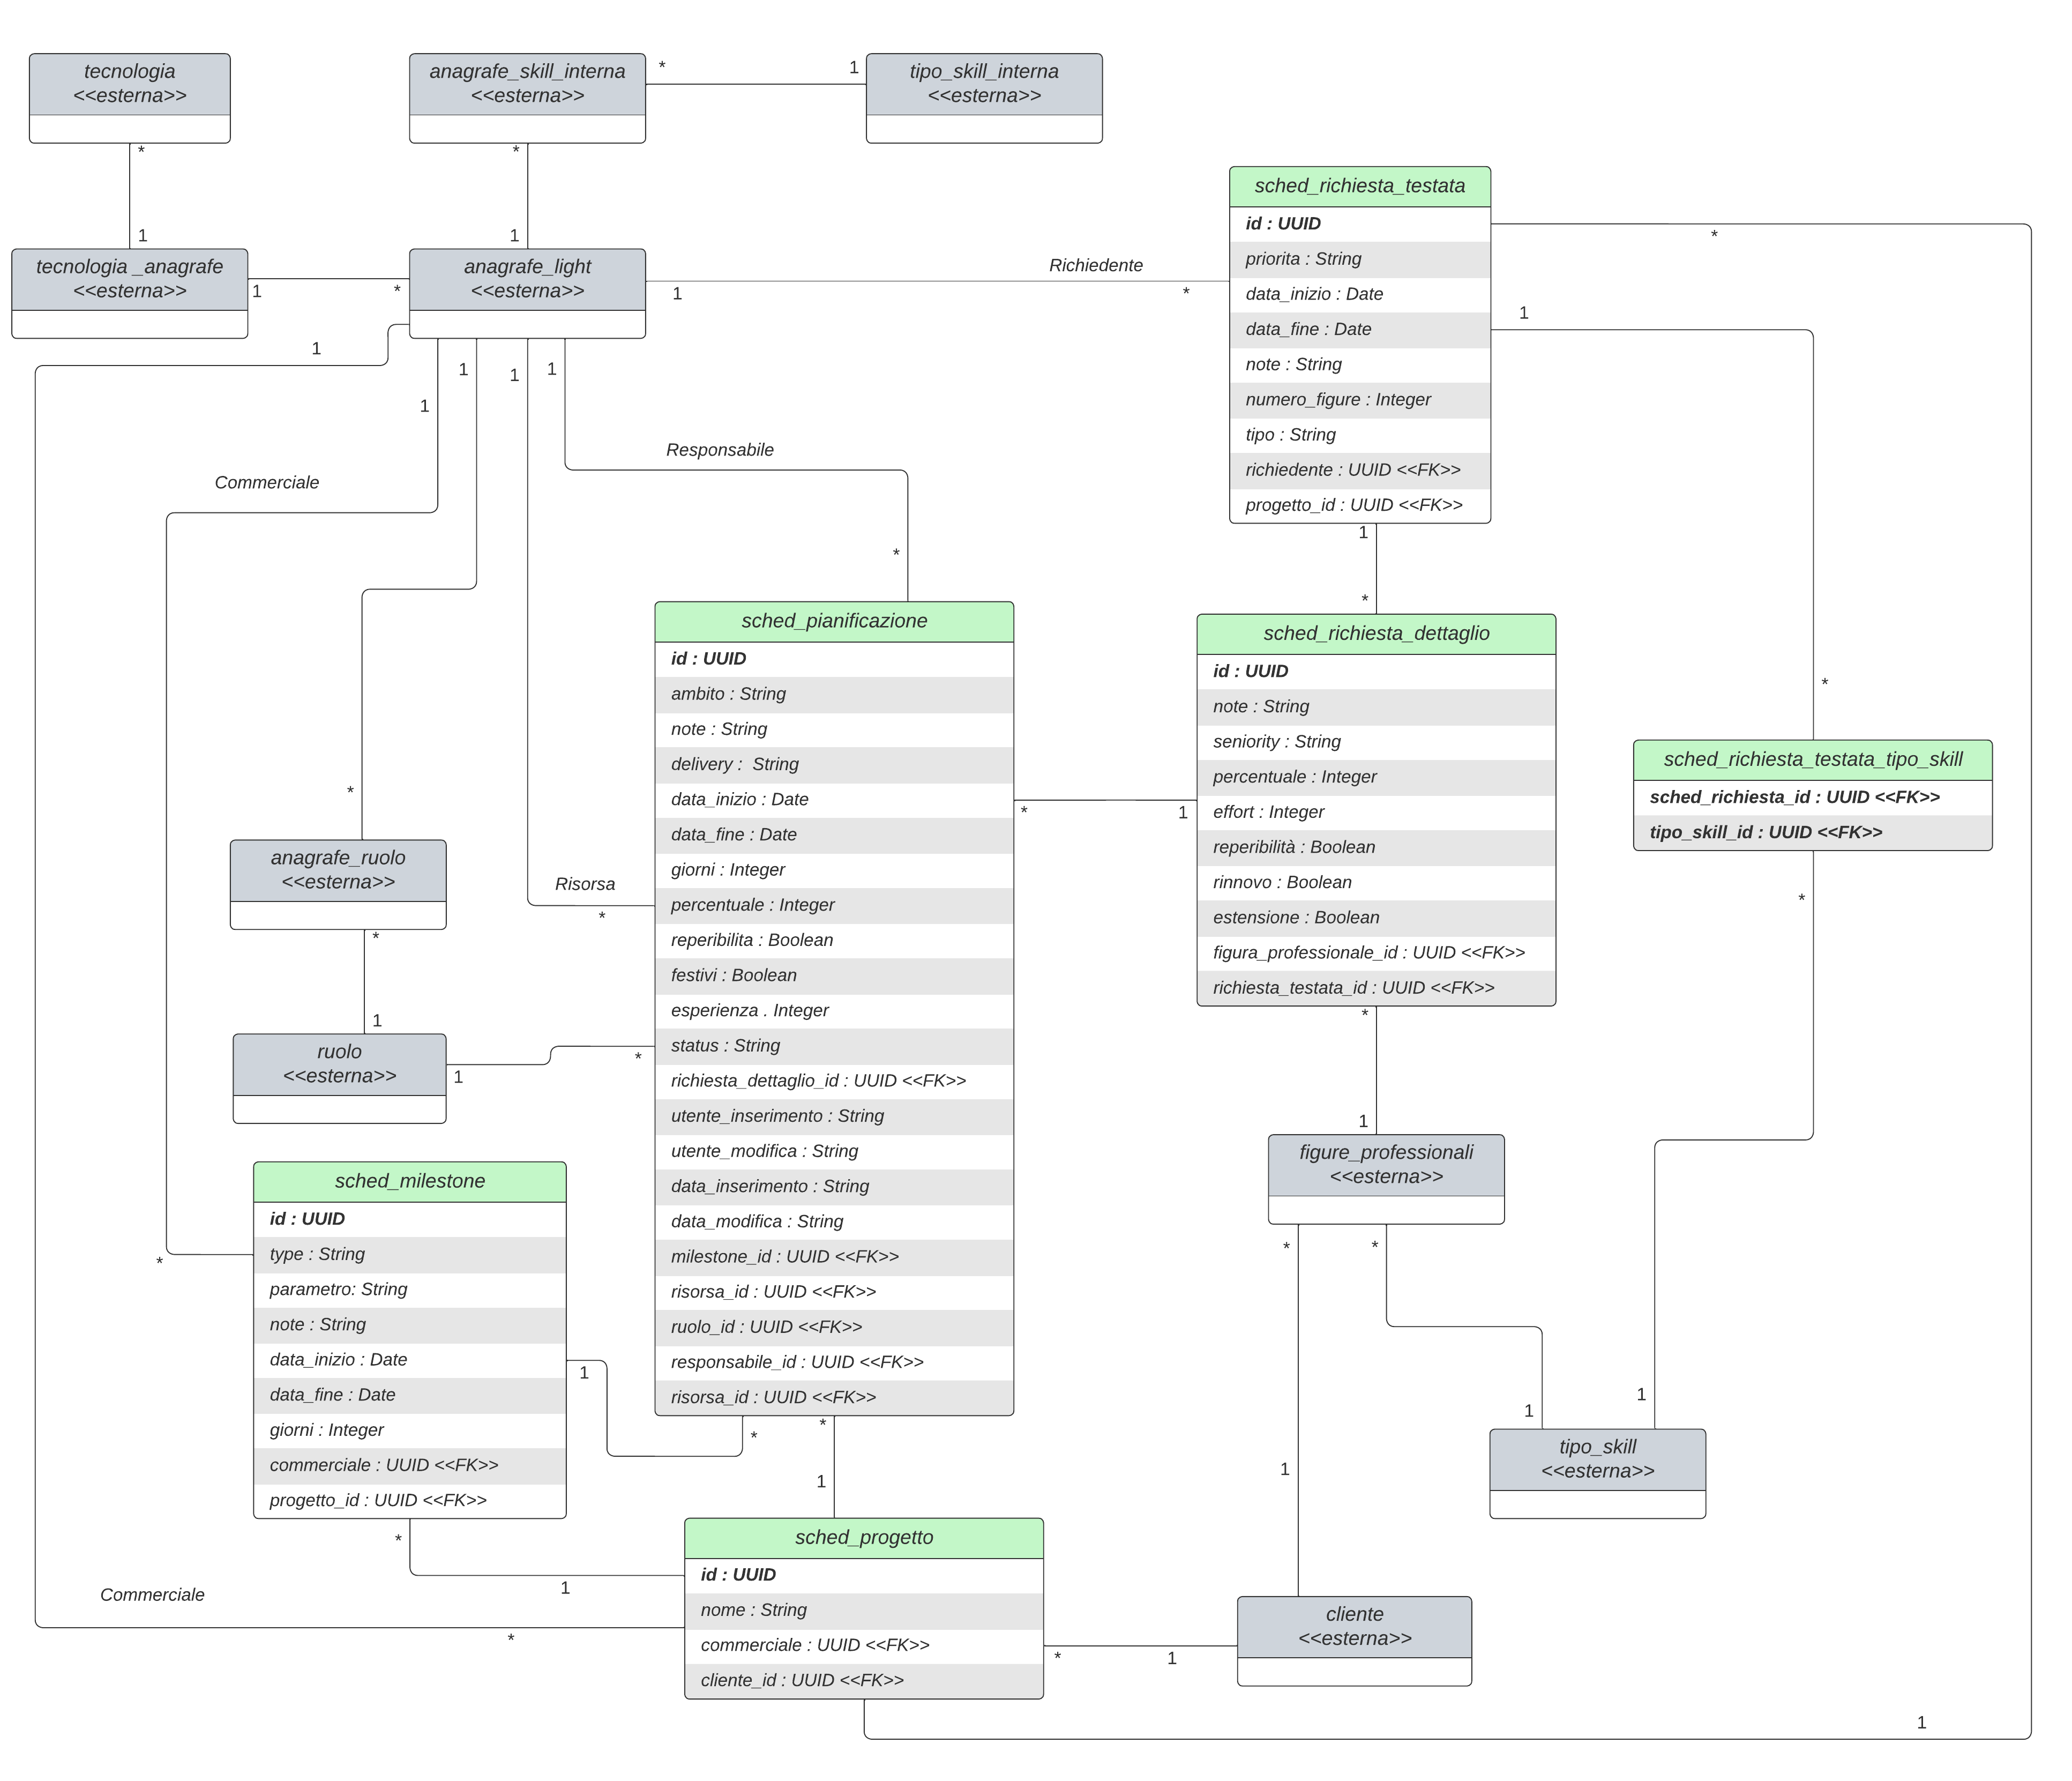
\includegraphics[width=1.2\columnwidth]{DB_Proj_noaudit} 
    \caption{Schema Database}
\end{figure}
\noindent Nel seguente disegno si può notare il database su cui poggia l'API.\\
È stata inserita una nomenclatura <<esterna>> per indicare le tabelle proveniente dal database aziendale. Per ogni tabella creata da me è stato deciso di utilizzare il prefisso "sched\_".\\
È stato utilizzato un UUID\textsubscript{g} come chiave primaria per ogni tabella.\\
Di seguito elenco l'utilizzo delle tabelle create da me e quelle del database aziendale, non trattando però gli attributi all'interno di quest'ultime:

\subsection*{tecnologia <<esterna>>}
Tabella del database aziendale utilizzata per mostrare le skill che una Risorsa possiede.
\subsection*{tecnologia\_anagrafe <<esterna>>}
Tabella di join del database aziendale tra la tabella contenente le anagrafiche aziendali e la tabella contenente le skill possedute da una Risorsa.
\subsection*{tipo\_skill\_interna <<esterna>>}
Tabella del database aziendale utilizzata per fornire le Aree di Competenza di ogni Risorsa.
\subsection*{anagrafe\_skill\_interna <<esterna>>}
Tabella di join del database aziendale tra la tabella \textit{tipo\_skill\_interna} e la tabella contenente le anagrafiche aziendali.
\subsection*{anagrafe\_light <<esterna>>} 
Tabella del database aziendale contenente i dati anagrafici di una Risorsa. All'interno del Database viene utilizzata questa tabella per prendere le informazioni in merito a: Richiedente della Richiesta, Responsabile della Pianificazione, Risorsa associata alla Pianificazione e Commerciale.
\subsection*{ruolo <<esterna>>}
Tabella del database aziendale contenente i ruoli possibili associati ad una Risorsa. Rappresenta il Ruolo che impiegherà nella Pianificazione.
\subsection*{anagrafe\_ruolo <<esterna>>}
Tabella di join del database aziendale tra \textit{anagrafe\_light} e \textit{ruolo}.
\subsection*{cliente <<esterna>>}
Tabella del database aziendale contenente i dati dei Clienti associabili ai Progetti.
\subsection*{sched\_progetto}
Tabella contenente i Progetti a cui una Richiesta o una Pianificazione può essere associata.

\setlength{\arrayrulewidth}{0.3mm}
\renewcommand{\arraystretch}{2.5}
\begin{center}
\rowcolors{1}{white}{mygray}
\begin{longtable}{p{3.7cm}|p{8.5cm}}
\textbf{Attributo}  & \textbf{Descrizione}\\
\hline
Id & UUID univoco <<PK>>\\
Nome & Nome del progetto\\
Commerciale & UUID del Commerciale associato <<FK>>\\
Cliente\_Id & UUID del Cliente associato <<FK>>\\
\hline
\hiderowcolors
\caption{Tabella sched\_progetto}
\label{tab:sched-progetto}
\end{longtable}
\end{center}

\subsection*{sched\_richiesta\_testata}
Tabella creata per gestire le Richieste create. Quando un Project Manager effettua una Richiesta creerà una nuova riga in questa tabella e nella tabella \textit{sched\_richiesta\_dettaglio} per ogni Figura Professionale richiesta. 

\setlength{\arrayrulewidth}{0.3mm}
\renewcommand{\arraystretch}{2.5}
\begin{center}
\rowcolors{1}{white}{mygray}
\begin{longtable}{p{3.7cm}|p{8.5cm}}
\textbf{Attributo}  & \textbf{Descrizione}\\
\hline
Id & UUID univoco <<PK>>\\
Priorità & Attributo che rappresenta la priorità (Alta,Media,Bassa)\\
Data\_inizio & Specifica la data di inizio per l'incarico richiesto\\
Data\_fine &  Specifica la data di fine per l'incarico richiesto\\
Note & Note inseribili dal Richiedente\\
Numero\_figure & Specifica il numero di figure richieste\\
Tipo & Specifica il tipo di attività richiesta\\
Richiedente & UUID del Richiedente della Richiesta <<FK>>\\
Progetto\_Id & UUID del Progetto associato <<FK>>\\
\hline
\hiderowcolors
\caption{Tabella sched\_richiesta\_testata}
\label{tab:sched-richiesta-testata}
\end{longtable}
\end{center}

\subsection*{sched\_richiesta\_testata\_tipo\_skill}
Tabella di join creata tra \textit{sched\_richiesta\_testata} e \textit{tipo\_skill}.\\
È stata creata per rappresentare la relazioni molti-a-molti tra le due tabelle.

\setlength{\arrayrulewidth}{0.3mm}
\renewcommand{\arraystretch}{2.5}
\begin{center}
\rowcolors{1}{white}{mygray}
\begin{longtable}{p{3.7cm}|p{8.5cm}}
\textbf{Attributo}  & \textbf{Descrizione}\\
\hline
sched\_richiesta\_id & Id della Richiesta associata <<PK>> <<FK>>\\
tipo\_skill\_id & Id della Skill richiesta associata <<PK>> <<FK>>\\
\hline
\hiderowcolors
\caption{Tabella sched\_richiesta\_testata\_tipo\_skill}
\label{tab:sched-richiesta-testata-tipo-skill}
\end{longtable}
\end{center}

\subsection*{tipo\_skill <<esterna>>}
Tabella del database aziendale contenente le skills conosciute o richiedibili alle Figure Professionali.

\subsection*{sched\_richiesta\_dettaglio}
Tabella creata per contenere i dettagli di ogni Figura richiesta. Ogni Figura richiesta corrisponde ad una nuova riga nella tabella.\\
È risultato obbligatorio utilizzare questo approccio per gestire la varietà di parametri assegnati per ogni figura richiesta dal Richiedente.

\setlength{\arrayrulewidth}{0.3mm}
\renewcommand{\arraystretch}{2.5}
\begin{center}
\rowcolors{1}{white}{mygray}
\begin{longtable}{p{3.7cm}|p{8.5cm}}
\textbf{Attributo}  & \textbf{Descrizione}\\
\hline
Id & UUID univoco <<PK>>\\
Note & Note inseribili per Figura\\
Seniority & Tipo di Seniority per ogni Figura (Junior, Middle, Senior)\\
Percentuale & Percentuale di impegno previsto per l'incarico\\
Effort & Quantità di impegno\\
Reperibilità & Booleano per indicare la reperibilità di una Figura\\
Rinnovo & Booleano per indicare il rinnovo dell'impegno della risorsa oltre la data indicata\\
Estensione & Booleano per che si riferisce all'estensione del lavoro sull'attività corrente\\
Figura\_professionale\_id & UUID della Figura Professionale associata <<FK>>\\
Richiesta\_testata\_id & UUID della Richiesta principale a cui è associata <<FK>>\\
\hline
\hiderowcolors
\caption{Tabella sched\_richiesta\_dettaglio}
\label{tab:sched-richiesta-dettaglio}
\end{longtable}
\end{center}

\subsection*{figure\_professionali <<esterna>>}
Tabella del database aziendale che contiene le Figure Professionali associabili ad una determinata skill richiesta.

\subsection*{sched\_pianificazione}
Tabella creata per contenere le Pianificazioni. Quando il Program Manager prende in carico una Richiesta posta dal Project Manager, per ogni Figura richiesta, ne crea una Pianificazione associando una Risorsa libera adeguata.

\setlength{\arrayrulewidth}{0.3mm}
\renewcommand{\arraystretch}{2.5}
\begin{center}
\rowcolors{1}{white}{mygray}
\begin{longtable}{p{3.7cm}|p{8.5cm}}
\textbf{Attributo}  & \textbf{Descrizione}\\
\hline
Id & UUID univoco <<PK>>\\
Ambito & Ambito di assegnazione della Pianificazione\\
Note & Note inseribili per la Pianificazione\\
Delivery & Valore che può essere Delivery Core (se riguarda aspetti fondamentali di un progetto) o Delivery Digital (se riguarda aspetti specifici di un progetto)\\
Data\_inizio & Data di inizio della Pianificazione\\
Data\_fine & Data di fine della Pianificazione\\
Giorni & Giorni di durata della Pianificazione\\
Percentuale & Indica la percentuale di impegno effettivo\\
Reperibilità & Booleano per indicare la reperibilità effettiva di una Figura\\
Festivi & Booleano per indicare l'opzione delle festività per una Figura\\
Esperienza & Intero rappresentante gli anni di esperienza\\
Status & Indica lo status della Pianificazione\\
Utente\_inserimento & Utente che ha inserito la Pianificazione\\
Utente\_modifica & Ultimo utente che ha modificato la Pianificazione\\
Data\_inserimento & Data di inserimento della Pianificazione\\
Data\_modifica & Ultima data di modifica della Pianificazione\\
Richiesta\_dettaglio\_id & UUID della Richiesta dettaglio associato <<FK>>\\
Milestone\_id & UUID della Milestone associata <<FK>>\\
Progetto\_id & UUID del Progetto associato <<FK>>\\
Ruolo\_id & UUID del Ruolo pianificato <<FK>>\\
Responsabile\_id & UUID del Responsabile associato <<FK>>\\
Risorsa\_id & UUID della Risorsa pianificata <<FK>>\\
\hline
\hiderowcolors
\caption{Tabella sched\_pianificazione}
\label{tab:sched-ianificazione}
\end{longtable}
\end{center}


\subsection*{sched\_milestone}
Tabella contenente i milestone associabili alla tabella delle Pianificazioni.\\
Una Milestone non può essere associata ad una Pianificazione se quest'ultima non è associata ad un Progetto.\\

\setlength{\arrayrulewidth}{0.3mm}
\renewcommand{\arraystretch}{2.5}
\begin{center}
\rowcolors{1}{white}{mygray}
\begin{longtable}{p{3.7cm}|p{8.5cm}}
\textbf{Attributo}  & \textbf{Descrizione}\\
\hline
Id & UUID univoco <<PK>>\\
Type & Indica il tipo di Milestone\\
Parametro & Specifica un'opzione personalizzata della Milestone\\
Note & Note inseribili per la Milestone\\
Data\_inizio & Data di inizio della Milestone\\
Data\_fine & Data di fine della Milestone\\
Giorni & Numero dei giorni di durata della Milestone\\
Commerciale & UUID del Commerciale associato <<FK>>\\
Progetto\_id & UUID del Progetto associato <<FK>>\\
\hline
\hiderowcolors
\caption{Tabella sched\_milestone}
\label{tab:sched-milestone}
\end{longtable}
\end{center}
